% ---------------------------- Preamble starts here ----------------------------

\documentclass[aspectratio=169]{beamer} %Remove [aspectratio=169] to get non-wide 4:3 slide aspect ratio

%-----------------------------------------------
% --- Set beamer theme
\usetheme{Metropolis}
\setbeamertemplate{footline}{}				% Remove automatic footer
\setbeamertemplate{navigation symbols}{}	% Comment this line to display navigation symbols

%-----------------------------------------------
% Load i2i symbol
\addtobeamertemplate{frametitle}{}{%
\begin{textblock*}{\linewidth}(0cm,7.4cm) % Replace with (0cm, 8cm) if using non-wide slide aspect
	\includegraphics[width=\linewidth]{../../Common-Resources/img/Footer.png}
\end{textblock*}}

%-----------------------------------------------
% --- Load packages
\usepackage{textpos}		% To align objects correctly
\usepackage{multicol}		% To right in multiple columns
\usepackage{color}			% To color text

%-----------------------------------------------
% --- Include link to last commit
\usepackage{xstring}
\usepackage{catchfile}

%Set this user input for link to commit
\newcommand{\gitfolder}{../../../.git} %relative path to .git folder from .tex doc
\newcommand{\reponame}{worldbank/dime-github-trainings} % Name of account and repo be set in URL

%Based on this https://tex.stackexchange.com/questions/455396/how-to-include-the-current-git-commit-id-and-branch-in-my-document
\CatchFileDef{\headfull}{\gitfolder/HEAD.}{} 				%Get path to head file for checked out branch
\StrGobbleRight{\headfull}{1}[\head]						%Remove end of line character
\StrBehind[2]{\head}{/}[\branch]							%Parse out the path only
\CatchFileDef{\commit}{\gitfolder/refs/heads/\branch.}{}	%Get the content of the branch head
\StrGobbleRight{\commit}{1}[\commithash]					%Remove end of line characted

%Build the URL to this commit based on the information we now have
\newcommand{\commiturl}{\url{https://github.com/\reponame/commit/\commithash}}

% Let's you add an image in line with a text
\newcommand*{\img}[1]{%
	\raisebox{-.3\baselineskip}{%
		\includegraphics[
		height=\baselineskip,
		width=\baselineskip,
		keepaspectratio,
		]{#1}%
	}%
}

%-----------------------------------------------
% --- Add your information here
\title{An intro to Git and GitHub - Contributor Role}
\author{Adopted by Sakina Shibuya from DIME Analytics}
\institute{DIME - The World Bank - \trainingURL{https://www.worldbank.org/en/research/dime}}
\date{October 26, 2022}

\newcommand{\trainingURL}[1]{{\color{blue}\url{#1}}}

\newcommand{\traininerUsername}{sakinashibuya}
\newcommand{\repoName}{\traininerUsername/lyrics_creb_F2022}
\newcommand{\trainingRepoURL}[1]{\trainingURL{https://github.com/\repoName #1}}
\newcommand{\trainerEmail}{\trainingURL{sshibuya2@wisc.edu} }


% ---------------------------- Preamble ends here ----------------------------

\begin{document}

\begin{frame}
\includegraphics[width=\textwidth]{../../Common-Resources/img/Header.png}
\vspace{-0.2cm}
\titlepage 	 % Opening slide, prints inform
\end{frame}

\begin{frame}
\frametitle{Before the session starts:}
	\begin{enumerate}
		\item Do you have a GitHub.com account? \\
		{\small $\rightarrow$ If not, got to \trainingURL{https://github.com/join} and sign up}
		\item Have you sent your GitHub username to the organizer at {\small \trainerEmail}?
		\item Have you installed GitHub Desktop? \\
		{\small $\rightarrow$ If not got to \trainingURL{https://desktop.github.com/} and download it.}
		\item Have you logged in at least once on GitHub Desktop? \\
		{\small $\rightarrow$ If not open GitHub Desktop and log in using your GitHub account.}
		\item Have you been invited to {\small \trainingRepoURL{}} ?
		\item And have you accepted at {\small \trainingRepoURL{/invitations}}?
	\end{enumerate}

\end{frame}


\begin{frame}
\frametitle{What is Git used for?}

	\begin{columns}[c]

		\column{.60\textwidth} % Left column and width
		\begin{itemize}
			\item Git solves \textbf{the \textit{Final.doc} problem}
			\begin{itemize}
				\item <2-> Commonly solved by naming all your docs like \textit{YYMMDD\_docname\_INITIALS.doc}
				\item <3-> \textbf{Git tracks \textit{YYMMDD} and \textit{INITIALS} for all edits  without the user having to remember it}
			\end{itemize}
			\item <4->That's far from everything, Git also solves:
			\begin{itemize}
				\item <4->Conflicting copy problem (DropBox etc.)
				\item <4->I can't re-produce my Baseline report problem
				\item <4->Who wrote this code 4 years ago and why?
				\item <4->And much much more...
			\end{itemize}
		\end{itemize}

		\column{.40\textwidth} % Right column and width
		\begin{figure}
			\centering
			\includegraphics[width=1\linewidth]{../../Common-Resources/img/finaldoc_cartoon}
			\label{fig:finaldoccartoon}
		\end{figure}

	\end{columns}
\end{frame}

\begin{frame}
	\frametitle{What is Git, GitHub and GitHub Desktop?}
	\begin{figure}
		\centering
		\includegraphics[width=0.85\linewidth]{../../Common-Resources/img/git_github_gitclient_git}
		\label{fig:gitgithubgitclient_git}
	\end{figure}
\end{frame}

\begin{frame}
	\frametitle{What is Git, GitHub and GitHub Desktop?}
	\begin{figure}
		\centering
		\includegraphics[width=0.85\linewidth]{../../Common-Resources/img/git_github_gitclient_github}
		\label{fig:gitgithubgitclient_github}
	\end{figure}
\end{frame}

\begin{frame}
	\frametitle{What is Git, GitHub and GitHub Desktop?}
	\begin{figure}
		\centering
		\includegraphics[width=0.85\linewidth]{../../Common-Resources/img/git_github_gitclient_gitclient}
		\label{fig:gitgithubgitclient_gitclient}
	\end{figure}
\end{frame}

\begin{frame}
	\frametitle{Three common GitHub roles}
	
	\small The objective of this training is to make you able to take the role of a \textbf{Contributor}. See DIME Analytics GitHub Roles for full details. (link at the end of the presentation)
	
	\input{../../Common-Resources/slides/GitHub-Roles.tex}
	
\end{frame}


\begin{frame}
\frametitle{What will we learn in this training?}

	In \textbf{An intro to Git and GitHub - Contributor Role} you will learn to:

	\begin{itemize}
		\setlength\itemsep{5mm}
		\item Explore the history of a project folder in GitHub and see what different team members are currently working on
		\item <2-> Three ways to interact with a repository:
		\begin{enumerate}
			\setlength\itemsep{2mm}
			\item <3-> \textbf{Clone}: Download a project folder from GitHub so you can work on 
			\item <4-> \textbf{Branch}: Create a space in the project folder where you can make your edits
			\item <5-> \textbf{Commit}: Make edits and share those versions with your team. When you are ready, request that your edits are included in the main version
		\end{enumerate}
	\end{itemize}
\end{frame}


\begin{frame}
\frametitle{Code-free training!}

	\begin{columns}[c]

		\column{.15\textwidth} % Left column and width

		\column{.70\textwidth} % Left column and width
		\textbf{No code today!}

		\vspace{.5cm}

		We will not work with code today.

		\vspace{.25cm}

		Code tends to distract people if, for example, they see a command they do not understand.

		\vspace{.25cm}

		Instead we will write simple lyrics on .txt files.

		\vspace{.25cm}
		
		This is an equivalent action to actual coding since Git read any text files.
		

		\column{.15\textwidth} % Left column and width

	\end{columns}
\end{frame}

\begin{frame}
\frametitle{How to browse GitHub.Com}

	A \textbf{repository} is a project folder in Git, often called \textbf{repo} for short.
	
	When you enter \trainingRepoURL{}, you get to what we will call the \textbf{repository landing page}.

	\vspace{.5cm}

	You can also go from \textbf{GitHub.com} to the \textbf{repo} of your choice.
	\begin{enumerate}
		\item From anywhere on \trainingURL{http://github.com}, click the \textit{octocat}  icon \img{img/octocat.png} in the top left corner.
		\item In the menu to your left, you see a list of repos you have access to.
		\item Click \textbf{\url{\repoName}} to get to the landing page.
	\end{enumerate}
	
\end{frame}

\section{Clone}

\begin{frame}
\frametitle{What is cloning?}

	Cloning is similar to \textbf{downloading a repository} to your computer.

	\vspace{.5cm}

	The difference between cloning and downloading is that \textbf{when Git clones a repository it remembers where you downloaded it from}. 

	\vspace{.5cm}
	
	This is necessary so that Git knows where to send any edits you make to the files, when sharing them with your team.

\end{frame}

\begin{frame}
\frametitle{How do I clone a repository from GitHub?}

	\begin{columns}[c]

		\column{.70\textwidth} % Left column and width
		How to clone a repository:
		\begin{enumerate}
			\setlength\itemsep{3mm}
			\item Go to the \textbf{landing page} of \trainingRepoURL{}
			\item Click the green \textit{Code} button (see image)
			\item Click \textit{Open with GitHub Desktop}
			\item Select where on your computer to clone the repository. \\
			\begin{itemize}
				\item \textbf{Do NOT clone in a shared folder, like a network drive or in Dropbox.} 
				\item Create a \textit{GitHub} folder in non-synced location and clone there.
			\end{itemize}
		\end{enumerate}

		\column{.30\textwidth} % Left column and width
		\begin{figure}
			\centering
			\includegraphics[width=1\linewidth]{img/clonedownload_button}
			\label{fig:clonedownloadbutton}
		\end{figure}

	\end{columns}

\end{frame}


\begin{frame}{Example: Where to store your repos on your device?}
	
	It's completely up to you, but here is that I do. 
	
	\begin{columns}[c]
		
		\column{.50\textwidth} % Left column and width
		
		\begin{itemize}
			\setlength\itemsep{3mm}
			\item Go to your \textbf{Documents} folder \\
			{\small PC: \path{C:\Users\sakina\Documents}} \\
			{\small Mac: \path{Home/Documents} or something}
			\item Create a new folder called \textbf{Github}.
			\item Note that this is NOT connected to any Cloud service like Box or Dropbox. 
		\end{itemize}
		
		\column{.50\textwidth} % Left column and width
		\begin{figure}
			\centering
			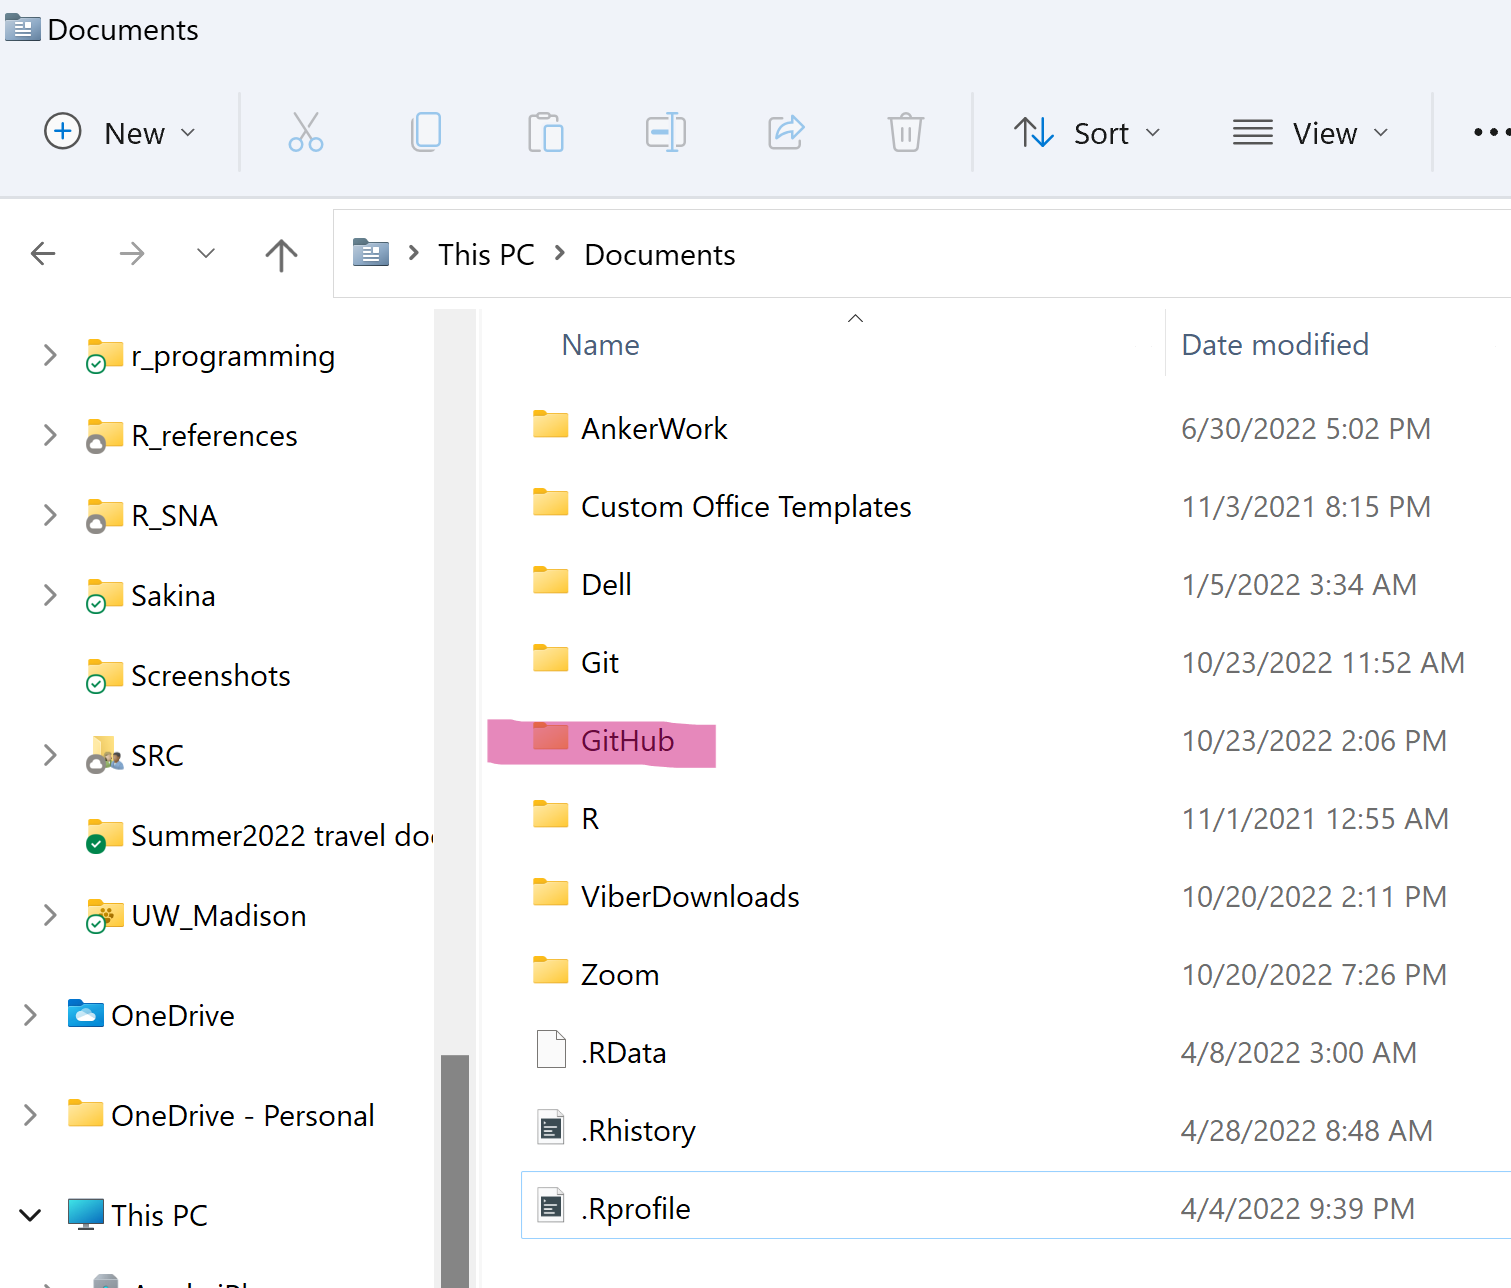
\includegraphics[width=\linewidth]{img/FolderExample}
			\label{fig:folderexample}
		\end{figure}

	\end{columns}	
\end{frame}


%\begin{frame}
%\frametitle{Explore the clone}
%
%	\begin{columns}[c]
%
%		\column{.20\textwidth} % Left column and width
%
%		\column{.60\textwidth} % Left column and width
%		\textbf{Explore the clone!}
%
%		\vspace{.5cm}
%
%		Compare the files and folders you cloned to your computer with those in the repository on \trainingRepoURL{}
%
%		\column{.20\textwidth} % Left column and width
%
%	\end{columns}
%
%\end{frame}

\section{Collaboration on a repository}

\begin{frame}
\frametitle{Collaboration needs two more concepts}

	\center{In order to collaborate on a repository we need to introduce two topics:}

	\vspace{1cm}

	\begin{columns}[c]

		\column{.30\textwidth} % Left column and width
		\center{\huge{\textbf{Commits}}}

		\column{.30\textwidth} % Left column and width
		\center{\huge{\textbf{Branches}}}

	\end{columns}

	\vspace{2cm}

\end{frame}

\section{Commit}

\begin{frame}
\frametitle{What is a version in version control?}

	\begin{columns}[c]

		\column{.50\textwidth}
		Dropbox is a very common tool of version control.
		
		\vspace{.5cm}
		
		How does Dropbox do it? \\
		$\rightarrow$ Each version is saved as an individual file in \textit{Version History}.
		
		\vspace{.5cm}
		
		Dropbox control versions automatically, but \textbf{are all these versions meaningful differences}?

		\column{.50\textwidth}
		\begin{figure}
			\centering
			\includegraphics[width=1\linewidth]{../../Common-Resources/img/dropbox_versioncontrol}
			\label{fig:dropboxversioncontrol}
		\end{figure}

	\end{columns}


\end{frame}

\begin{frame}
\frametitle{What is a commit?}

	Instead of having a list of each saved version of a file, \textbf{Git uses commits to indicate each meaningful difference between two versions of our project folder}.

	\vspace{.25cm}

	Each commit is: 
	\begin{itemize}
		\item a snap shot of all files in the project folder,
		\item a list of differences across the snap shots (the previous commits).
	\end{itemize}

	\vspace{.25cm}

	Each commit tracks \textbf{when} and \textbf{who}. \\
	{\small $\rightarrow$ This is very similar to the \textit{YYMMDD\_docname\_INITIALS.doc} solution to the \textit{Final.doc} problem.} 

\end{frame}

\begin{frame}
\frametitle{How to make a commit}

	We need to introduce \textit{branches} before we can all commit to the same repository, so for now, let me show you how to make a commit:

	\begin{enumerate}
		\item I add a new text file in the clone
		\item I use GitHub desktop to commit the new file to the repository
		\item Can you see the new file on your computer?
		\item Can you see it if you sync in GitHub Desktop?
	\end{enumerate}

\end{frame}


\begin{frame}
\frametitle{Exploring commits}

	Now when we know what a commit is, we can start exploring how the \trainingRepoURL{} repository was created.

	\vspace{.25cm}

	We will see a list of commits, that at first sight is similar to the the version history in DropBox, but \textbf{in Git the version list is more meaningful, as it is a list of only meaningful differences}.

	\vspace{.25cm}

	\begin{itemize}
		\item \trainingRepoURL{/commits}
		\item This list can also be found in GitHub Desktop in the \textit{History} tab
	\end{itemize}

\end{frame}

\section{Branch}

\begin{frame}
\frametitle{Introducing branches, the ``killer feature" of Git}

	\begin{columns}[c]

		\column{.60\textwidth}
	
		\textbf{A \textit{branch} is a copy of the repo where you can experiment} without disturbing what your teammates are doing. 
		
		\vspace{.5cm}
		
		If you like the result, \textbf{you can very easily merge your experiment with the main version of your repo}.

		\vspace{.5cm}

		This non-linear version control is much more similar to how we actually work than the strictly linear version control in, for example, Dropbox.

		\column{.40\textwidth}
		\begin{figure}
			\centering
			\includegraphics[width=1\linewidth]{../../Common-Resources/img/branches}
			\label{fig:branches}
		\end{figure}

	\end{columns}

\end{frame}


\begin{frame}
\frametitle{How to create a branch on Github.com}

	\begin{itemize}
		\setlength\itemsep{3mm}
		\item Go to \trainingRepoURL{}
		\item Click the button, \textit{main}.
		\item Write your name in the field and click \textit{Create branch: YourName}. Make sure it says \textit{from 'main'}.
		\item See how the button now says \textit{YourName}
		\item Go to \trainingRepoURL{/network} to check that your branch is there.
	\end{itemize}

\end{frame}


\begin{frame}
	\frametitle{How to create a branch from GitHub Desktop}
	
	\begin{itemize}
		\item Go to \url{\repoName}
		\item Click the tab, \textit{Current branch main}
		\item Write your name in the field and click \textit{New Branch}
		\item Hit \textit{Create Branch} in the pop-up window
		\item See the tab now says \textit{Current branch YourName}
		\item Publish your branch by clicking \textit{Publish branch}
		\item Go to \trainingRepoURL{/network} to check that your branch is there
	\end{itemize}
	
\end{frame}



\section{Combining Commit \& Branch}

\begin{frame}
\frametitle{Now it is time to collaborate}

\textbf{Now it is time for you to collaborate:}
\begin{enumerate}
	\item Make sure your branch is checked out in GitHub Desktop.
	\item Open a text editor. 
	\begin{itemize}
		\item Windows: \textit{Notepad}
		\item Mac: \textit{TextEdit}
		\item Feel free to use whatever text editor you want.
	\end{itemize}
	\item Type a sentence. (e.g. Hello, my name is Sakina!)
	\item Save the lyrics in your local clone according to these instructions:
	\begin{itemize}
		\item Save the file in \textit{.txt} format \\
		{\small \textbf{Mac users}, this is not always the default.}
		\item Name the file after the title of the song
		\item Save it in your local repo folder
	\end{itemize}
\end{enumerate}

\end{frame}

\begin{frame}
\frametitle{Do your first commit}

\begin{columns}[c]

\column{.60\textwidth} % Left column and width

\begin{enumerate}
	\item Open the changes tab in GitHub Desktop
	\item GitHub Desktop tracks your clone and has noticed that you changed something in it
	\item Then you need to do the three steps required to commit a file to the repository:
	\begin{enumerate}
		\item Make sure the file you want to add is checked
		\item Write a commit message
		\item Click \textit{Commit to your\_name} - check out your branch if it says \textit{main}
		\item Click the sync button
	\end{enumerate}
\end{enumerate}

\column{.40\textwidth} % Left column and width
\begin{figure}
	\centering
	\includegraphics[width=1\linewidth]{img/desktop_changes}
	\label{fig:desktopchanges}
\end{figure}

\vspace{-1cm}

\begin{figure}
	\centering
	\includegraphics[width=1\linewidth]{img/desktop_commit}
	\label{fig:desktop_commit}
\end{figure}

\end{columns}

\end{frame}

\begin{frame}
\frametitle{Check your contribution}

	\textbf{Check your commit on GitHub:}
	\begin{itemize}
		\item Go to \trainingRepoURL{/network}
		\begin{itemize}
			\item Can you find your commit?
		\end{itemize}
		\item Go to \trainingRepoURL{/commits}
		\begin{itemize}
			\item Can you find your commit?
			\item If you cannot see your commit, make sure that you are looking in the correct branch
		\end{itemize}
	\end{itemize}

\end{frame}

\begin{frame}
	\frametitle{Looking at branches}
	
	
	\textbf{One more way to explore the repository}
	\begin{itemize}
		\item \trainingRepoURL{/commits} $<$- Linear progression
		\item \trainingRepoURL{/network} $<$- Non-linear progression
	\end{itemize}
	
	\vspace{.1cm}
	
	\textbf{Exploring branches}
	\begin{itemize}
		\item You can change branch in \textit{/commits}. What happens when you change branch?
		\item Go to the landing page, what happens if you change branch here?
		\item Which version is in the clone on your computer? They are all actually in your clone, but only one is shown - \textbf{checked out} - at the time
		\item What happens to the content of the folder on your computer when you check out another branch in GitHub Desktop?
	\end{itemize}
	
\end{frame}

\begin{frame}
\frametitle{Merging branches to the \textit{main} branch}

	A contributor can do this by submitting a \textbf{pull request}.
	
	\vspace{0.25cm}
	\textbf{When to submit a pull request}	
	You should do this when you are done with your experiment, and satisfied with the outcome.
	
	\vspace{0.25cm}
	\textbf{Who can make a pull request:}
	A pull request can be made either by the person that edited the branch or the repo maintainer.
	
	\vspace{0.25cm}
	
	It is a common practice that only the repo maintainer have access to the main branch, and pull requests are then the only way to contribute to the main branch.


\end{frame}

\begin{frame}
\frametitle{Merge your contribution}

	\textbf{To make a pull request for your branch:}
	\begin{itemize}
		\item Go to \trainingRepoURL{/pulls}
		\item Click \textit{New pull request}
		\item Make sure that the \textit{main} branch is selected as the \textit{base:} branch
		\item Select \textbf{your} branch as the \textit{compare:} branch
		\item Check the edits you are requesting to be pulled in to the main branch. 
		\item Click \textit{Create pull request} if you are ok with the edits
		\item Add comments and instructions about your edits
		\item Click \textit{Create pull request} again
	\end{itemize}
\end{frame}

\begin{frame}
\frametitle{Merge your contribution}

Go to \trainingRepoURL{} to see if you see your edits.

You won't see them because rour contribution will not be included \textbf{until the branch is merged}. 

More training on the details of merging branches in \textcolor{blue}{\url{https://github.com/sakinashibuya/git_training_creb_F2022}} for your reference.

But for now, all you need to know is the following:
	\begin{itemize}
		\item Always have someone to review your PR before merging it
		\item Always delete your branch after it is merged - you can always recreate a new branch with the same name if you want
	\end{itemize}

\end{frame}

\begin{frame}
	\frametitle{How to merge}
	
	\vspace{3cm}
	
	\textbf{For now, let me just show you how to do this.}
	
	\vspace{3cm}
\end{frame}

%\begin{frame}
%\frametitle{What have we learned?}
%
%	In \textbf{An intro to Git and GitHub - Contributor Role} you have learned to:
%
%	\begin{itemize}
%		\item Explore the history of a project folder in GitHub and see what different team members are currently working on
%		\item Download a project folder from GitHub so you can work on it
%		\item Create a space in the project folder where you can make your edits
%		\item Make edits and share those versions with your team. When you are ready, request that your edits are included in the main version
%	\end{itemize}
%
%\end{frame}

\begin{frame}
\frametitle{What have we learned?}

	In \textbf{An intro to Git and GitHub - Contributor Role} you have learned to:

	\begin{itemize}
		\item Explore the history of \textbf{repository} and see what different team members are currently working on
		\item \textbf{Clone} a \textbf{repository} so you can work on it
		\item Create a \textbf{branch} in the \textbf{repository} where you can make your edits
		\item Make edits and share \textbf{commits} with your team. When you are ready, make a \textbf{pull request} to the \textbf{main branch}
	\end{itemize}
\end{frame}


\section{Next steps for the research team}

\begin{frame}
\frametitle{Three common GitHub Roles}

	\input{../../Common-Resources/slides/GitHub-Roles.tex}

\end{frame}

\begin{frame}
\frametitle{Next steps for the research team}

	Before adopting Git the research team should discuss the following things:

	\begin{itemize}
		\item Who will be repo maintainer
		\item Agree on a work flow
		\item Public/private repository
		\item External collaborators
		\item Where to put data and where to put code
		\item Request a repo on DIME or World Bank account
	\end{itemize}

\end{frame}

\input{../../Common-Resources/slides/GitHub-Links.tex}

\input{../../Common-Resources/slides/GitHub-Commit-URL.tex}


\end{document}
